\documentclass[11pt, oneside]{article}
\usepackage[margin=.9in]{geometry}
\usepackage{pgfplots}
\pgfplotsset{compat=default}
\newcommand{\cuckoo}{{\rm cuckoo}}
\newcommand{\hash}{{\rm siphash}}
\usepackage{hyperref}
\usepackage{listings}
\title{Cuckoo Cycle: \protect\\ a memory-bound graph-theoretic proof-of-work system}
\author{John Tromp}
\begin{document}
\maketitle

\begin{abstract}
We introduce the first graph-theoretic proof-of-work system,
based on finding small cycles or other structures in large random graphs.
Such problems are trivially verifiable and arbitrarily scalable, 
appearing to require memory linear in graph size to solve efficiently.
Our cycle finding algorithm uses one bit per edge, and up to one bit per node.
Runtime is linear in graph size and dominated by random access latency,
ideal properties for a memory-bound proof-of-work.
We exhibit two alternative algorithms that allow for a memory-time trade-off
(TMTO)---decreased memory usage, by a factor $k$, coupled with increased runtime, by a factor $\Omega(k)$.
The constant implied in $\Omega()$ gives a notion of memory-hardness, which is shown to be dependent
on cycle length, guiding the latter's choice. Our algorithms are shown to parallelize reasonably well.
\end{abstract}

\section{Introduction}
A ``proof of work'' (PoW) system allows a verifier to check with negligible
effort that a prover has expended a large amount of computational effort.
Originally introduced as a spam fighting measure, 
where the effort is the price paid by an email sender for demanding the
recipient's attention, they now form one of the cornerstones of crypto-currencies.

As proof-of-work for new blocks of transactions,
Bitcoin~\cite{nakamoto2009bitcoin} adopted Adam Back's hashcash~\cite{back2002} proof-of-work.
This entails finding a nonce value such that application of a cryptographic hash function
to this nonce and the rest of the block header, results in a number below a
target threshold\footnote{or, less accurately, results in many leading 0s}.
The threshold is dynamically adjusted by the protocol
so as to maintain an average block interval of 10 minutes.

Bitcoin's choice of the simple and purely compute-bound SHA256 hash function
allowed for an easy migration of hash computation from 
desktop processors (CPUs) to graphics-card processors (GPUs),
to field-programmable gate arrays (FPGAs), and finally to custom designed
chips (ASICs), with huge improvements in energy-efficiency at every step.

Since Bitcoin, many other crypto-currencies have adopted hashcash, with various
choices of underlying hash function. the most well-known being {\em scrypt} as
introduced by Tenebrix~\cite{tenebrix2011}---which since faded into obscurity---and
copied by Litecoin~\cite{litecoin2011}.
Scrypt, designed as a sequential memory-hard key derivation function,
was specifically chosen to resist the migration away from CPUs and be ``GPU-hostile''.
However, to adapt to the efficient verifiability requirement of proof-of-work, its
memory footprint was severely limited, and migration slowed down only slightly.

Primecoin~\cite{king2013} introduced the notion of a number-theoretic proof-of-work,
thereby offering the first alternative to hashcash among crypto-currencies.
Primecoin identifies long chains of nearly doubled prime numbers, constrained
by a certain relation to the block header.
Verification of these chains, while very slow compared to bitcoin's, is much faster
than attempting to find one.
This asymmetry between proof (attempt) and verification is typical in non-hashcash proofs of work.
Recently, another prime-number based crypto-currency, Riecoin, was introduced, based
on finding clusters rather than chains of prime numbers.

Momentum~\cite{larimer2013} proposes finding birthday collisions of hash outputs,
in what could well be the simplest possible assymetric proof-of-work,
combining scalable memory usage with trivial verifiability.
In section~\ref{cycle_length_choice} we show that Momentum is in essence a special case of Cuckoo Cycle,
one that is particularly susceptible to time-memory tradeoffs.

Adam Back~\cite{back2014} has a good overview of proof-of-work papers past and present.

\section{Motivation}
Cuckoo Cycle aims to be an ``egalitarian'' proof-of-work, that is, to minimize performance differences
across hardware architectures. This is best achieved by making memory latency the bottleneck, since
main memory latencies have remained relatively stable, while cpu-speed and memory bandwidth are highly
variable across both time and architecture.

We thus aim to have a memory footprint that exceeds a single memory-chip, to minimize the amount
of computation in between random memory accesses, and making any tradeoff of memory for time
incur a substantial penalty.

The above aims should apply only to proof attempts---the real work---but not to proof verification,
which ideally requires negligable memory and time. Thus, we aim for a highly assymetric design.
A final aim is to keep the design very simple.

We do not aim to have provable lower bounds on memory usage. Such bounds appear to be
attainable only under the so called {\em random oracle model}, where memory tends to be used
merely as a store for chains of outputs of some compute-intensive hash function.
Instead we will present a ``reference'' efficient proof-finding algorithm,
along with our best attempts at memory-time tradeoffs,
and conjecture that these cannot be significantly improved upon.
In that sense, this work is more empirical than formal.

\section{Graph-theoretic proofs-of-work}
We propose to base proofs-of-work on finding certain subgraphs in large pseudo-random graphs.
In the Erd\H{o}s-R\'{e}nyi model, denoted $G(N,M)$, a graph is chosen uniformly at random
from the collection of all graphs with $N$ nodes and $M$ edges. Instead, we choose edges
deterministically from the output of a keyed hash function, whose key could be chosen
uniformly at random. For a well-behaved hash function, these two classes of random graphs
should have nearly identical properties.

Formally, fix a keyed hash function
$h: \{0,1\}^K \times \{0,1\}^{W_i} \rightarrow \{0,1\}^{W_o}$,
and a small graph $H$ as a target subgraph\footnote{hash functions generally have arbitrary length inputs,
but here we fix the input width at $W_i$ bits.}.
Now pick a large number $N \leq 2^{W_o}$ as the number of nodes,
and $M \leq 2^{W_i-1}$ as the number of edges.
Each key $k \in \{0,1\}^K$ generates a graph $G_k = (V,E)$ where $V=\{v_0,\ldots,v_{N-1}\}$, and
\begin{equation}
E=\{(v_{h(k,2i) \bmod N},v_{h(k,2i+1) \bmod N}) | i \in [0,\ldots,M-1]\}
\end{equation}
The inputs $i \in [0,\ldots,M-1]$ are also called {\em nonces}\footnote{These
{\em micro} nonces should be distinguished from the {\em macro} nonce used to generate key $k$.}
The graph has a {\em solution} if $H$ occurs as a subgraph.
Denote the number of edges in $H$ as $L$.
A proof of solution is an ordered list of $L$ nonces that generate the edges
of $H$'s occurrence in $G_k$.
Such a proof is verifiable in time depending only on $H$ (typically linear in $L$), independent of $N$ and $M$.

A simple variation generates random bipartite graphs: $G_k = (V_0 \cup V_1,E)$ where (assuming $N$ is even)
$V_0=\{v_0,v_2,\ldots,v_{N-2}\}$, $V_1=\{v_1,v_3,\ldots,v_{N-1}\}$, and
\begin{equation}
\label{hash_edges}
E=\{(v_{2(h(k,2i) \bmod \frac{N}{2})}, v_{2(h(k,2i+1) \bmod \frac{N}{2})+1}) | i \in [0,\ldots,M-1]\}
\end{equation}

The expected number of occurrences of $H$ as a subgraph of $G$ is a function of both $N$ and $M$,
and in many cases is roughly a function of $\frac{M}{N}$ (half the average node degree).
For fixed $N$, this function is monotonically increasing in $M$.
To make the proof-of-work challenging, one chooses a value of $M$ that yields less than one
expected solution.

The simplest possible choice of subgraph is a fully connected one, or a {\em clique}.
While an interesting choice, akin to the number-theoretic notion of a prime-cluster,
as used in Riecoin, we leave its consideration to a future paper.

\section{Cuckoo Cycle}
In this paper we focus on what is perhaps the next-simplest possible choice, the {\em cycle}.
Specifically, we propose the hash function \hash\ with a $K=128$ bit key, $W_i = W_o = 64$ input
and output bits, $N \leq 2^{64}$ a 2-power, $M=N/2$, and $H$ an $L$-cycle.
The reason for calling the resulting proof-of-work Cuckoo Cycle is that
inserting items in a Cuckoo hashtable naturally leads to cycle formation
in random bipartite graphs.

\section{Cuckoo hashing}
Introduced by Rasmus Pagh and Flemming Friche
Rodler~\cite{Pagh04cuckoohashing}, a Cuckoo hashtable consists of two
same-sized tables each with its own hash function mapping a key to a table
location, providing two possible locations for each key.
Upon insertion of a new key, if both locations are already occupied by keys,
then one is kicked out and inserted in its alternate location, possibly
displacing yet another key, repeating the process until either a vacant
location is found, or some maximum number of iterations is reached.
The latter is bound to happen once cycles have formed in the {\em Cuckoo graph}.
This is a bipartite graph with a node for each location and an
edge for every inserted key, connecting the two locations it can reside at.
It matches the bipartite graph defined above if the cuckoo hashtable
were based on function $h$.
In fact, the insertion procedure suggests a simple algorithm for detecting cycles.

\section{Cycle detection in Cuckoo Cycle}
We enumerate the $M$ nonces, but instead of storing the nonce itself as a key
in the Cuckoo hashtable, we store the alternate key location,
and forget about the nonce.  We thus maintain the {\em directed}
cuckoo graph, in which the edge for a key is directed from the location where
it resides to its alternate location.  Moving a key to its alternate location
thus corresponds to reversing its edge.  The outdegree of every node in this
graph is either 0 or 1.  When there are no cycles yet, the graph is a {\em
forest}, a disjoint union of trees.  In each tree, all edges are directed,
directly, or indirectly, to its {\em root}, the only node in the tree with
outdegree 0.  Initially there are just $N$ singleton trees consisting of
individual nodes which are all roots.
Addition of a new key causes a cycle if and only if its two endpoints are
nodes in the same tree, which we can test by following the path from each
endpoint to its root.
In case of different roots, we reverse all edges on the shorter of the two
paths, and finally create the edge for the new key itself, thereby joining
the two trees into one. Let us illustrate this process with an actual example.

The left diagram in Figure~\ref{cycleformation} shows the directed cuckoo graph for header ``39'' on
$N=8+8$ nodes after adding edges
$(2,15),(4,9),(8,5),(4,15),(12,11),(10,5)$ and $(4,13)$ (nodes
with no incident edges are omitted for clarity).
In order to add the 8th edge $(10,11)$, we follow the paths $10 \rightarrow 5
\rightarrow 8$ and $11 \rightarrow 12$ to find different roots $8$ and $12$.
Since the latter path is shorter, we reverse it to $12 \rightarrow 11$ so we
can add the new edge as $(11 \rightarrow 10)$, resulting in the middle diagram.
In order to add to 9th edge
$(10,13)$ we now find the path from $10$ to be the shorter one, so we reverse
that and add the new edge as $(10 \rightarrow 13)$, resulting in the right diagram.
\begin{figure}
\begin{center}
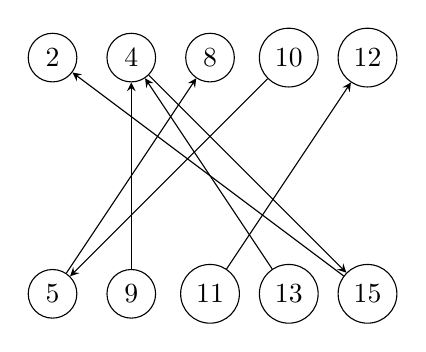
\begin{tikzpicture}[>=stealth]
\node  (2) at (1, 2) [shape=circle,draw] {2};
\node  (4) at (2, 2) [shape=circle,draw] {4};
\node  (8) at (3, 2) [shape=circle,draw] {8};
\node (10) at (4, 2) [shape=circle,draw] {10};
\node (12) at (5, 2) [shape=circle,draw] {12};
\node  (5) at (1,-1) [shape=circle,draw] {5};
\node  (9) at (2,-1) [shape=circle,draw] {9};
\node (11) at (3,-1) [shape=circle,draw] {11};
\node (13) at (4,-1) [shape=circle,draw] {13};
\node (15) at (5,-1) [shape=circle,draw] {15};
\draw [<-]  (2) -- (15);
\draw [<-]  (4) -- (9);
\draw [<-]  (8) -- (5);
\draw [->]  (4) -- (15);
\draw [<-] (12) -- (11);
\draw [->] (10) -- (5);
\draw [<-]  (4) -- (13);
\end{tikzpicture}\hspace{1cm}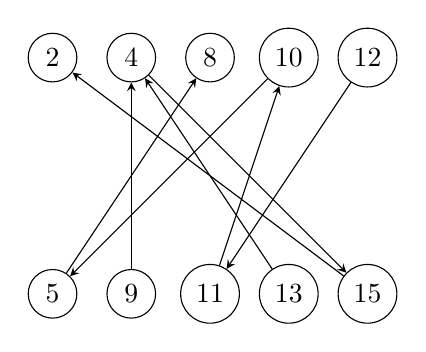
\begin{tikzpicture}[>=stealth]
\node  (2) at (1, 2) [shape=circle,draw] {2};
\node  (4) at (2, 2) [shape=circle,draw] {4};
\node  (8) at (3, 2) [shape=circle,draw] {8};
\node (10) at (4, 2) [shape=circle,draw] {10};
\node (12) at (5, 2) [shape=circle,draw] {12};
\node  (5) at (1,-1) [shape=circle,draw] {5};
\node  (9) at (2,-1) [shape=circle,draw] {9};
\node (11) at (3,-1) [shape=circle,draw] {11};
\node (13) at (4,-1) [shape=circle,draw] {13};
\node (15) at (5,-1) [shape=circle,draw] {15};
\draw [<-]  (2) -- (15);
\draw [<-]  (4) -- (9);
\draw [<-]  (8) -- (5);
\draw [->]  (4) -- (15);
\draw [->] (12) -- (11);
\draw [->] (10) -- (5);
\draw [<-]  (4) -- (13);
\draw [<-] (10) -- (11);
\end{tikzpicture}\hspace{1cm}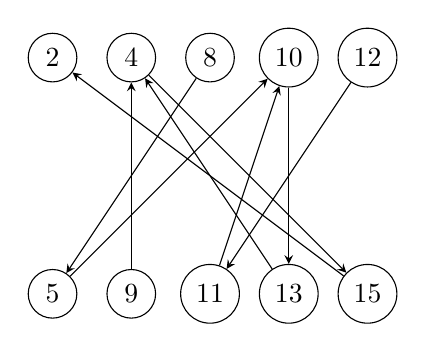
\begin{tikzpicture}[>=stealth]
\node  (2) at (1, 2) [shape=circle,draw] {2};
\node  (4) at (2, 2) [shape=circle,draw] {4};
\node  (8) at (3, 2) [shape=circle,draw] {8};
\node (10) at (4, 2) [shape=circle,draw] {10};
\node (12) at (5, 2) [shape=circle,draw] {12};
\node  (5) at (1,-1) [shape=circle,draw] {5};
\node  (9) at (2,-1) [shape=circle,draw] {9};
\node (11) at (3,-1) [shape=circle,draw] {11};
\node (13) at (4,-1) [shape=circle,draw] {13};
\node (15) at (5,-1) [shape=circle,draw] {15};
\draw [<-]  (2) -- (15);
\draw [<-]  (4) -- (9);
\draw [->]  (8) -- (5);
\draw [->]  (4) -- (15);
\draw [->] (12) -- (11);
\draw [<-] (10) -- (5);
\draw [<-]  (4) -- (13);
\draw [<-] (10) -- (11);
\draw [->] (10) -- (13);
\end{tikzpicture}
\end{center}
\caption{Cycle Formation}
\label{cycleformation}
\end{figure}
When adding the 10th edge $(8,9)$, we find the paths $8 \rightarrow 5
\rightarrow 10 \rightarrow 13 \rightarrow 4 \rightarrow 15 \rightarrow 2$ and
$9 \rightarrow 4 \rightarrow 15 \rightarrow 2$ with equal roots.
In this case, we can compute the length of the resulting cycle as
1 plus the sum of the path-lengths to the node where the two paths join.
In the diagram, the paths join at node $4$, and the cycle length is computed as $1+4+1=6$.

\section{Union-find}
The above representation of the directed cuckoo graph is an example of
a {\em disjoint-set data structure}~\cite{wikidsds2014}, and our algorithm is
closely related to the well-known union-find algorithm, where the find operation
determines which subset an element is in, and the union operation joins two subsets
into a single one. For each edge addition to the cuckoo graph we perform the equivalent
of two find operations and one union operation.
The difference is that the union-find algorithm is free to add
directed edges between arbitrary elements. Thus it can join two subsets by adding an edge
from one root to another, with no need to reverse any edges.
Our algorithm on the other hand solves the union-find problem by maintaining
a direction on all union operations while keeping the maximum outdegree at 1.

\section{Cuckoo Cycle basic algorithm}
The above algorithm for inserting edges and detecting cycles forms the basis
for our basic proof-of-work algorithm.
If a cycle of length $L$ is found, then we solved the problem, and recover the proof
by storing the cycle edges in a set and enumerating nonces once more to see which ones
generate edges in the set.
If a cycle of a different length is found, then we keep the graph acyclic by ignoring the edge.
There is some risk of overlooking other $L$-cycles
through that edge, but when the expected number of cycles is low (which is what we design for),
this ignoring of cycle forming edges hardly affects the rate of solution finding.

This algorithm is available online at \url{https://github.com/tromp/cuckoo}
as either the C-program simple\_miner.cpp or the Java program SimpleMiner.java.
A proof verifier is available as cuckoo.c or Cuckoo.java, while the repository
also has a Makefile, as well as the latest version of this paper.
% `make test' tests everything.
`make example' reproduces the example shown above.
The simple program uses 32 bits per node to represent the directed cuckoo graph,
plus about 64KB per thread for two path-following arrays.
The left plot in Figure~\ref{runtimes} shows both the total runtime in seconds and the runtime of just
the hash computation, as a function of (log)size. The latter is purely
linear, while the former is superlinear due to increasing memory latency
as the nodes no longer fit in cache. The right plot show this more clearly
as the percentage of hashing to total runtime, ending up around 5\%.

\begin{figure}
\begin{center}
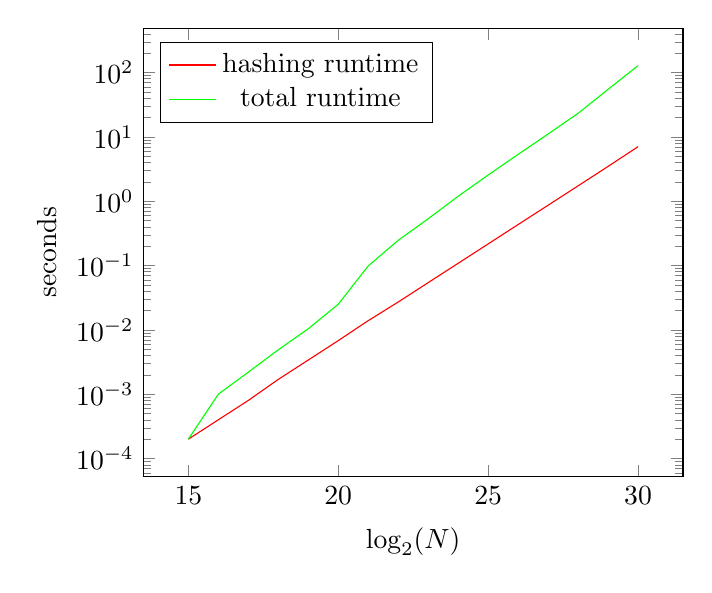
\begin{tikzpicture}
\begin{axis}[xlabel={$\mbox{log}_2(N)$}, ymode=log, ylabel={seconds}, legend pos=north west]
\addplot[color=red] coordinates {
% (10,0.0000) (11,0.0000) (12,0.0000) (13,0.0001) (14,0.0001)
(15,0.0002) (16,0.0004) (17,0.0008) (18,0.0017) (19,0.0034)
(20,0.0068) (21,0.0139) (22,0.0271) (23,0.0542) (24,0.1084)
(25,0.2166) (26,0.4336) (27,0.8658) (28,1.7322) (29,3.4719)
(30,7.0389) };
\addlegendentry{hashing runtime}
\addplot[color=green] coordinates {
% (10,0.0000) (11,0.0000) (12,0.0001) (13,0.0001) (14,0.0003)
(15,0.0002) (16,0.0010) (17,0.0022) (18,0.0049) (19,0.0104)
(20,0.0250) (21,0.0986) (22,0.2465) (23,0.5332) (24,1.1922)
(25,2.5505) (26,5.3394) (27,11.0793) (28,23.1984) (29,54.6811)
(30,128.1682) };
\addlegendentry{total runtime}
\end{axis}
\end{tikzpicture}
% \hspace{1mm}
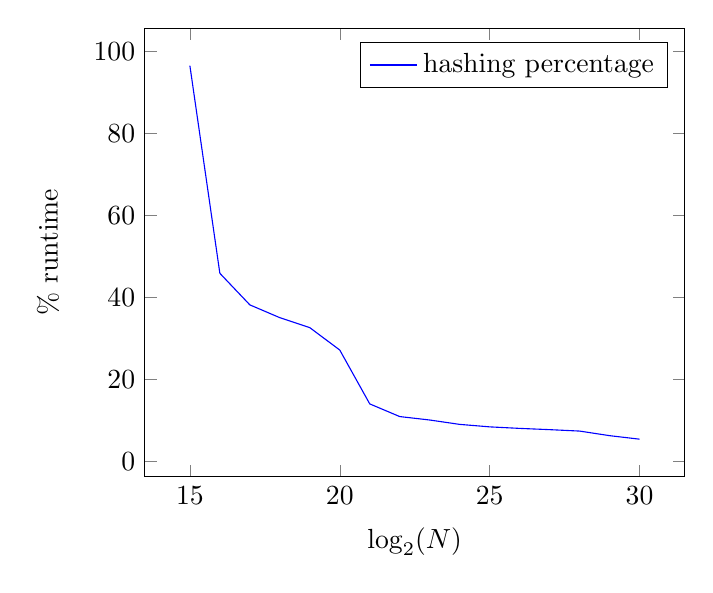
\begin{tikzpicture}
\begin{axis}[xlabel={$\mbox{log}_2(N)$}, ylabel={\% runtime}, legend pos=north east]
\addplot[color=blue] coordinates {
% (10,38.8889) (11,33.3333) (12,45.1613) (13,39.8496) (14,44.6154)
(15,96.5217) (16,45.9119) (17,38.2180) (18,35.0988) (19,32.6724)
(20,27.2076) (21,14.0874) (22,11.0014) (23,10.1635) (24,9.0964)
(25,8.4921) (26,8.1215) (27,7.8144) (28,7.4670) (29,6.3494)
(30,5.4919) };
\addlegendentry{hashing percentage}
\end{axis}
\end{tikzpicture}
\end{center}
\caption{Runtime}
\label{runtimes}
\end{figure}

The left plot in Figure~\ref{accesses} shows the probability of finding a 42-cycle as a function
of the percentage edges/nodes, while the right plot shows the average number of
memory reads and writes per edge as a function of the percentage
of processed nonces (progress through main loop).
Both were determined from 10000 runs at size $2^{20}$;
results at size $2^{25}$ look almost identical.
In total the basic algorithm averages 3.3 reads and 1.1 writes per edge.

\begin{figure}
\begin{center}
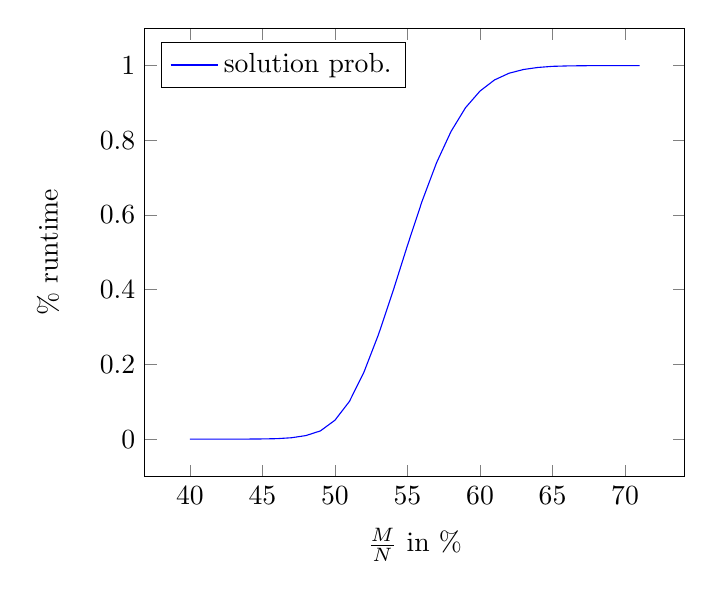
\begin{tikzpicture}
\begin{axis}[xlabel={$\frac{M}{N}$ in \%}, ylabel={\% runtime}, legend pos=north west]
\addplot[color=blue] coordinates {
(40,0) (41,0.00001) (42,0.00003) (43,0.0001) (44,0.00031) (45,0.00067)
(46,0.00141) (47,0.00385) (48,0.00967) (49,0.02222) (50,0.05076)
(51,0.10117) (52,0.17953) (53,0.27993) (54,0.39581) (55,0.51873)
(56,0.63614) (57,0.73955) (58,0.82352) (59,0.88719) (60,0.93182)
(61,0.9616) (62,0.97949) (63,0.98956) (64,0.99503) (65,0.99799)
(66,0.99907) (67,0.9996) (68,0.99989) (69,0.99997) (70,0.99998) (71,1) };
\addlegendentry{solution prob.}
\end{axis}
\end{tikzpicture}
% \hspace{1cm}
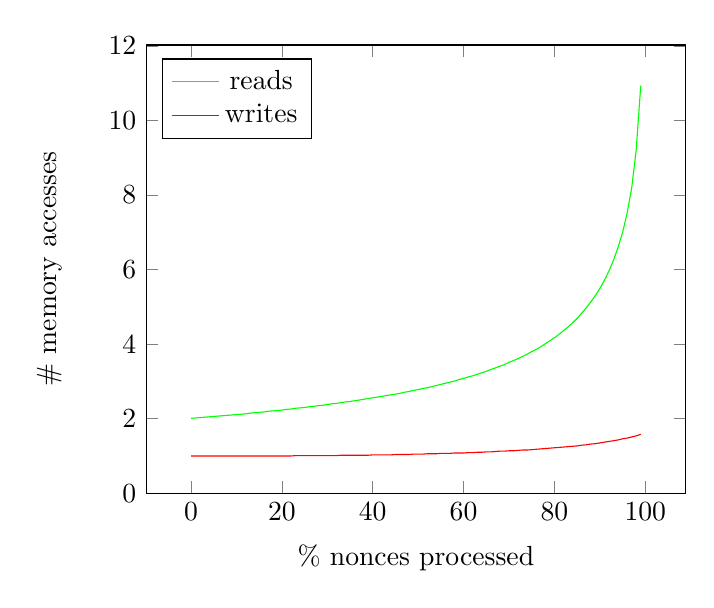
\begin{tikzpicture}
\begin{axis}[xlabel={\% nonces processed}, ylabel={\# memory accesses}, ymin=0, legend pos=north west]
\addplot[color=green] coordinates {
(0,2.01) (1,2.02) (2,2.03) (3,2.04) (4,2.05) (5,2.06) (6,2.07) (7,2.08) (8,2.09) (9,2.10) (10,2.11) (11,2.12) (12,2.13) (13,2.15) (14,2.16) (15,2.17) (16,2.18) (17,2.20) (18,2.21) (19,2.22) (20,2.23) (21,2.25) (22,2.26) (23,2.28) (24,2.29) (25,2.30) (26,2.32) (27,2.33) (28,2.35) (29,2.36) (30,2.38) (31,2.40) (32,2.41) (33,2.43) (34,2.45) (35,2.46) (36,2.48) (37,2.50) (38,2.52) (39,2.54) (40,2.56) (41,2.58) (42,2.60) (43,2.62) (44,2.64) (45,2.66) (46,2.68) (47,2.71) (48,2.73) (49,2.76) (50,2.78) (51,2.81) (52,2.83) (53,2.86) (54,2.89) (55,2.92) (56,2.95) (57,2.98) (58,3.01) (59,3.05) (60,3.08) (61,3.12) (62,3.15) (63,3.19) (64,3.23) (65,3.27) (66,3.32) (67,3.36) (68,3.41) (69,3.45) (70,3.51) (71,3.56) (72,3.61) (73,3.67) (74,3.73) (75,3.80) (76,3.86) (77,3.93) (78,4.01) (79,4.09) (80,4.17) (81,4.26) (82,4.36) (83,4.46) (84,4.57) (85,4.69) (86,4.83) (87,4.97) (88,5.13) (89,5.30) (90,5.49) (91,5.71) (92,5.96) (93,6.25) (94,6.59) (95,6.99) (96,7.51) (97,8.18) (98,9.20) (99,10.93) };
\addlegendentry{reads}
\addplot[color=red] coordinates {
(0,1.00) (1,1.00) (2,1.00) (3,1.00) (4,1.00) (5,1.00) (6,1.00) (7,1.00) (8,1.00) (9,1.00) (10,1.00) (11,1.00) (12,1.00) (13,1.00) (14,1.00) (15,1.00) (16,1.00) (17,1.00) (18,1.00) (19,1.00) (20,1.00) (21,1.00) (22,1.00) (23,1.01) (24,1.01) (25,1.01) (26,1.01) (27,1.01) (28,1.01) (29,1.01) (30,1.01) (31,1.01) (32,1.01) (33,1.02) (34,1.02) (35,1.02) (36,1.02) (37,1.02) (38,1.02) (39,1.02) (40,1.03) (41,1.03) (42,1.03) (43,1.03) (44,1.03) (45,1.04) (46,1.04) (47,1.04) (48,1.04) (49,1.05) (50,1.05) (51,1.05) (52,1.06) (53,1.06) (54,1.06) (55,1.07) (56,1.07) (57,1.07) (58,1.08) (59,1.08) (60,1.08) (61,1.09) (62,1.09) (63,1.10) (64,1.10) (65,1.11) (66,1.11) (67,1.12) (68,1.13) (69,1.13) (70,1.14) (71,1.14) (72,1.15) (73,1.16) (74,1.16) (75,1.17) (76,1.18) (77,1.19) (78,1.20) (79,1.21) (80,1.22) (81,1.23) (82,1.24) (83,1.25) (84,1.26) (85,1.27) (86,1.29) (87,1.30) (88,1.32) (89,1.33) (90,1.35) (91,1.37) (92,1.39) (93,1.41) (94,1.43) (95,1.46) (96,1.48) (97,1.51) (98,1.54) (99,1.58) };
\addlegendentry{writes}
\end{axis}
\end{tikzpicture}
\end{center}
\caption{Memory acceses}
\label{accesses}
\end{figure}

\section{Difficulty control}
The ratio $\frac{M}{N}$ determines a base level of difficulty,
which may suffice for applications where difficulty is to remain fixed.
Ratios $\frac{M}{N} \geq 0.7$ are suitable when a practically guaranteed solution is desired.

For crypto currencies, where difficulty must scale in precisely
controlled manner across a large range, adjusting the number of edges is not suitable.
The implementation default $\frac{M}{N}=\frac{1}{2}$ gives a solution probability of roughly $2.2\%$,
while the average number of cycles found increases slowly with size; from 2 at $2^{20}$
to 3 at $2^{30}$.

For further control, a difficulty target $0 < T < 2^{256}$ is introduced,
and we impose the additional constraint that the sha256 digest of the
cycle nonces in ascending order be less than $T$, thus
reducing the success probability by a factor $\frac{2^{256}}{T}$.

\section{Edge Trimming}
\label{edge_trimming}
David Andersen~\cite{dga2014} suggested drastically reducing the number of edges
our basic algorithm has to process, by repeatedly identifying nodes of degree one
and eliminating their incident edge. Such {\em leaf edges} can never be part of a cycle.
This works well when $\frac{M}{N} \leq \frac{1}{2}$ since the expected degree of a node is then at most 1,
and a significant fraction of edges are expected to be leaf edges.

Trimming is implemented in our main algorithm in cuckoo\_miner and hcuckoo\_miner.cpp.
It maintains a set of {\em alive} edges as a bit vector. Initially all edges are alive.
In each of a given number of trimming rounds, it shrinks this set as follows.
A vector of 2-bit degree counters, one per even node, is initialized to all zeroes.
Next, for all alive edges, compute its even endpoint and increase the corresponding counter,
capping the value at 2.
Next, for all alive edges, compute its even endpoint and if the corresponding counter is less than 2,
set the edge to be not-alive.
These steps are repeated for all odd endpoints.

Preprocessor symbol PART\_BITS, whose value we'll denote as $B$,
allows for {\em counter partitioning}, which trades off node counter storage for runtime,
by processing nodes in multiple passes depending on the value of their $B$ least significant
bits\footnote{excluding the very least significant bit distinguishing even from odd nodes.}.
The memory usage is $M$ bits for the alive set and $N / 2^{B}$ for the counters.

The diagrams in Figure~\ref{trimming} show two rounds of edge trimming on the earlier example. In round one
even nodes 2 and 12 lose their single incident edge and in round two, odd nodes 11 and 15 lose
their remaining single incident edge. At this point only the 6-cycle is left, so further trimming
would be pointless.

\begin{figure}
\begin{center}
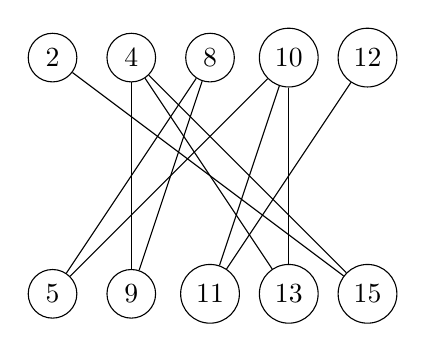
\begin{tikzpicture}[>=stealth]
\node  (2) at (1, 2) [shape=circle,draw] {2};
\node  (4) at (2, 2) [shape=circle,draw] {4};
\node  (8) at (3, 2) [shape=circle,draw] {8};
\node (10) at (4, 2) [shape=circle,draw] {10};
\node (12) at (5, 2) [shape=circle,draw] {12};
\node  (5) at (1,-1) [shape=circle,draw] {5};
\node  (9) at (2,-1) [shape=circle,draw] {9};
\node (11) at (3,-1) [shape=circle,draw] {11};
\node (13) at (4,-1) [shape=circle,draw] {13};
\node (15) at (5,-1) [shape=circle,draw] {15};
\draw [-]  (2) -- (15);
\draw [-]  (4) -- (9);
\draw [-]  (8) -- (5);
\draw [-]  (4) -- (15);
\draw [-] (12) -- (11);
\draw [-] (10) -- (5);
\draw [-]  (4) -- (13);
\draw [-] (10) -- (11);
\draw [-] (10) -- (13);
\draw [-]  (8) -- (9);
\end{tikzpicture}\hspace{1cm}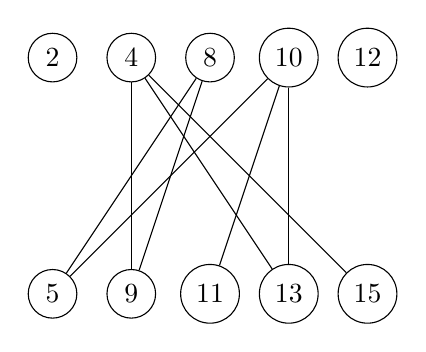
\begin{tikzpicture}[>=stealth]
\node  (2) at (1, 2) [shape=circle,draw] {2};
\node  (4) at (2, 2) [shape=circle,draw] {4};
\node  (8) at (3, 2) [shape=circle,draw] {8};
\node (10) at (4, 2) [shape=circle,draw] {10};
\node (12) at (5, 2) [shape=circle,draw] {12};
\node  (5) at (1,-1) [shape=circle,draw] {5};
\node  (9) at (2,-1) [shape=circle,draw] {9};
\node (11) at (3,-1) [shape=circle,draw] {11};
\node (13) at (4,-1) [shape=circle,draw] {13};
\node (15) at (5,-1) [shape=circle,draw] {15};
\draw [-]  (4) -- (9);
\draw [-]  (8) -- (5);
\draw [-]  (4) -- (15);
\draw [-] (10) -- (5);
\draw [-]  (4) -- (13);
\draw [-] (10) -- (11);
\draw [-] (10) -- (13);
\draw [-]  (8) -- (9);
\end{tikzpicture}\hspace{1cm}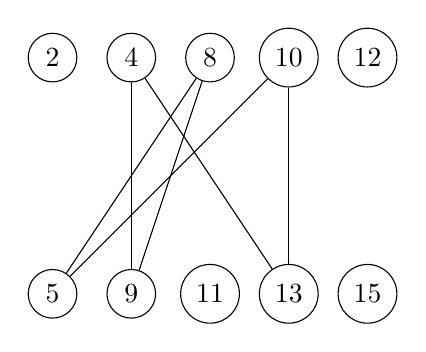
\begin{tikzpicture}[>=stealth]
\node  (2) at (1, 2) [shape=circle,draw] {2};
\node  (4) at (2, 2) [shape=circle,draw] {4};
\node  (8) at (3, 2) [shape=circle,draw] {8};
\node (10) at (4, 2) [shape=circle,draw] {10};
\node (12) at (5, 2) [shape=circle,draw] {12};
\node  (5) at (1,-1) [shape=circle,draw] {5};
\node  (9) at (2,-1) [shape=circle,draw] {9};
\node (11) at (3,-1) [shape=circle,draw] {11};
\node (13) at (4,-1) [shape=circle,draw] {13};
\node (15) at (5,-1) [shape=circle,draw] {15};
\draw [-]  (4) -- (9);
\draw [-]  (8) -- (5);
\draw [-] (10) -- (5);
\draw [-]  (4) -- (13);
\draw [-] (10) -- (13);
\draw [-]  (8) -- (9);
\end{tikzpicture}
\end{center}
\caption{Edge Trimming}
\label{trimming}
\end{figure}

After all edge trimming rounds, the counter memory is freed, and allocated to a
custom cuckoo\_hashtable (based on \cite{preshing2013}) that presents the same interface as the
simple array in the basic algorithm, but gets by with much fewer locations, as long as its {\em load},
the ratio of remaining edges to number of locations, is bounded away from 1; e.g. under 90 percent.

The number of trimming rounds, which can be set with option {\tt -n}, defaults to
$1+(B+3)*(B+4)/2$, which was determined empirically to achieve a load close to $50\%$.

\section{Time-Memory Trade-Offs (TMTOs)}
David Andersen also suggested an alternative method of trimming that avoids storing a bit per edge.
Expanding on that idea led to the algorithm implemented in tomato\_miner.h,
which, unlike the main algorithm, can trade-off memory directly for runtime.
On the downside, to even achieve memory parity with the main algorithm, it already incurs a big slowdown.
To the extent that this slowdown is unavoidable, it can be called the {\em memory hardness} of the proof-of-work.

The TMTO algorithm selects a suitably small subset $Z$ of even vertices as a base layer,
and on top of that builds a breadth-first-search
(BFS) forest of depth $L/2$, i.e. half the cycle length.
For each new BFS layer, it enumerates all edges to see which ones are incident
to the previous layer, adding the other endpoint.
It maintains a directed forest on all BFS nodes, like the base algorithm does on all nodes.
For increased efficiency, the base layer $Z$ is filtered for nodes with multiple incident edges.
If the graph has an $L$-cycle one of whose nodes is in $Z$, then the above procedure will find it.
If one choice of $Z$ doesn't yield a solution, then the data structures are cleared and the next
subset is tried.

A variation on the above algorithm omits the filtering of $Z$, and expands
the BFS to a whole $L$ levels. This way, an $L$-cycle will be found as long as the distance from (any node in)
$Z$ to the cycle is at most $L/2$. It thus has a much higher chance of finding a cycle, but requires
more space to store the significantly bigger BFS forest.

For each each value of $L \in \{2,4,6,8,10,12,14,16,20,24,28,32,40,48,56,64\}$ we ran these 2 algorithms
on 200 graphs of size $2^{25}$ that include an $L$-cycle,
choosing subset size as a 2-power that results in a memory usage of 4MB,
and analysed the distribution of number of subsets tried before
finding a solution. Since there is possible overlap between the BFS forests of different initial subsets,
especially with the second algorithm, the distributions are skewed toward lower numbers. To maximize solution
finding rate then, it pays to give up on a graph when the first few subsets tried fail to provide a solution.
For each algorithm and cycle length, we determined the minimum number of tries needed to guarantee solutions
in at least 50 of the 200 graphs. In Figure~\ref{slowdown} we plot the slowdown relative to the reference algorithm also using 4MB
(2MB for edges and 2MB for nodes).

\begin{figure}
\begin{center}
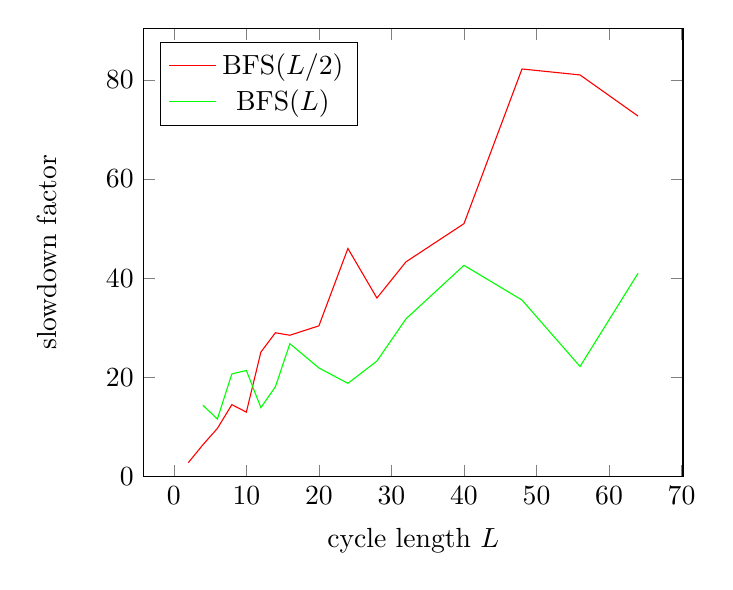
\begin{tikzpicture}
% \begin{axis}[ymin=0, xtick={2,8,16,24,32,40,48,56,64}, xlabel={cycle length $L$}, ylabel={slowdown factor}, legend pos=north west]
\begin{axis}[ymin=0, xlabel={cycle length $L$}, ylabel={slowdown factor}, legend pos=north west]
\addplot [color=red] coordinates {
(2,2.8) (4,6.4) (6,9.7) (8,14.5) (10,13.0) (12,25.1) (14,29.0) (16,28.5)
(20,30.4) (24,46.0) (28,36.0) (32,43.3) (40,51.0) (48,82.2) (56,81.0) (64,72.7)
};
\addlegendentry{BFS($L/2$)}
\addplot [color=green] coordinates {
(4,14.4) (6,11.6) (8,20.7) (10,21.4) (12,13.9) (14,18.1) (16,26.8) (20,21.9)
(24,18.8) (28,23.3) (32,31.8) (40,42.6) (48,35.6) (56,22.2) (64,41.0)
};
\addlegendentry{BFS($L$)}
%\addplot [color=blue, mark=o] coordinates {
%(2, 1.4)
%};
%\addlegendentry{customized}
\addlegendentry{}
\end{axis}
\end{tikzpicture}
\end{center}
\caption{Slowdown}
\label{slowdown}
\end{figure}

The zigzagging is caused by the current implementation being limited to 2-power sizes of
both subsets and cuckoo tables while the load of the latter is kept between 45\% and 90\%\footnote{We
plan to lift this restriction in the near future and produce smoother plots with constant load cuckoo tables.}
The BFS($L$) algorithm exhibits at least one order of magnitude slowdown, that grows very slowly
with cycle length, while the BFS($L/2$) algorithm exhibits roughly linear slowdown.
Assuming that these algorithms cannot be significantly improved upon, we obtain an order of magnitude
memory hardness for Cuckoo Cycle with larger cycle lengths.

\section{Choice of cycle length}
\label{cycle_length_choice}
A cycle of length 2 means that two nonces produce identical edge endpoints---a {\em collision} in edge space.
The Momentum proof-of-work looks for collisions on 50 bits of hash output among $2^{26}$ nonces.
This is in essence Cuckoo Cycle with $N=2^{25}+2^{25}$ nodes and cycle length $L=2$, with
two differences.

First, edges are generated not by equation~(\ref{hash_edges}), but by splitting a SHA512 hash of
$(k,\mbox{nonce} / 8)$ into 8 64-bit words, taking the most significant 50 bits of the
($\mbox{nonce} \bmod 8)th$ one, and viewing that as a pair of two 25-bit edge endpoints, appending
a bit to make them even and odd.

Second, the choice of $M=2^{26}$ gives a ratio $\frac{M}{N}$ of 1 rather than $\frac{1}{2}$ and as such
prohibits the use of edge trimming.

Since the extreme case of $L=2$ is so special, there is likely to be a greater variety of algorithms that are more
efficient than for the general case. While we haven't found (and don't know of) a improved main algorithm,
we did find an improved BFS($L/2$) TMTO algorithm (implemented in momentomatum.cpp)
that cuts the memory usage in half, resulting in a slowdown of only $1.75$---a lack of memory-hardness.

The preceding analysis suggests that cycle length should be at least 20 to guard against the more efficient
BFS($L/2$) algorithm, with an additional safety factor of 2.

In order to keep proof size manageable, the cycle length should not be too large either.
We thus consider 20-64 to be a healthy range, and suggest the use of the average of 42.

The plot below shows the distribution of cycle lengths found for sizes $2^{10},2^{15},2^{20},2^{25}$,
as determined from 100000,100000,10000, and 10000 runs respectively. The tails of the distributions
beyond $L=100$ are not shown. For reference, the longest cycle found was of length 2120.

\begin{figure}
\begin{center}
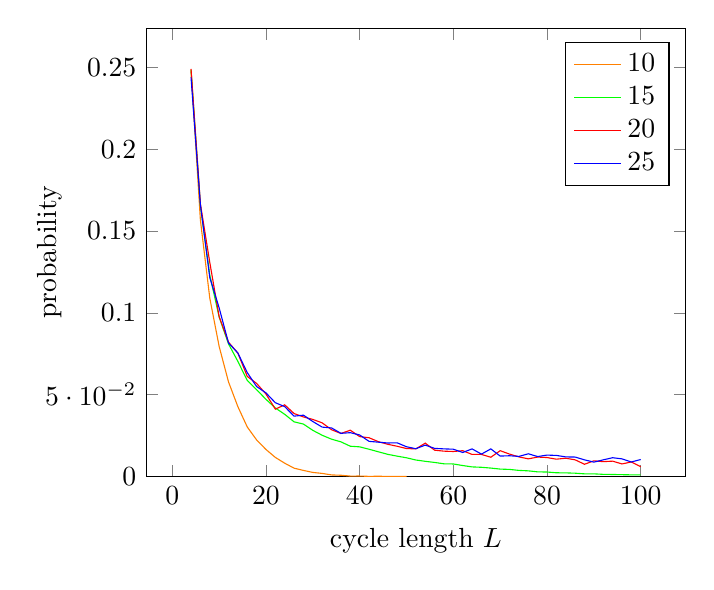
\begin{tikzpicture}
\begin{axis}[ymin=0, xlabel={cycle length $L$}, ylabel={probability}, legend pos=north east]
\addplot[color=orange] coordinates {
(4,0.24862) (6,0.15673) (8,0.10907) (10,0.07952) (12,0.05783) (14,0.04269) (16,0.0303)
(18,0.02237) (20,0.01653) (22,0.01168) (24,0.00815) (26,0.00511) (28,0.00374) (30,0.00251)
(32,0.00191) (34,0.00098) (36,0.00079) (38,0.00029) (40,0.0003) (42,0.00011) (44,0.00018)
(46,8e-05) (48,2e-05) (50,3e-05) };
\addlegendentry{10}
\addplot[color=green] coordinates {
(4,0.24822) (6,0.16551) (8,0.12317) (10,0.09749) (12,0.08105) (14,0.07036) (16,0.05871) (18,0.05308)
(20,0.04717) (22,0.04189) (24,0.03801) (26,0.03342) (28,0.03205) (30,0.02822) (32,0.02521)
(34,0.02282) (36,0.0212) (38,0.01852) (40,0.01814) (42,0.01668) (44,0.01511) (46,0.01356)
(48,0.01246) (50,0.01145) (52,0.0101) (54,0.0093) (56,0.00861) (58,0.00778) (60,0.00768)
(62,0.00672) (64,0.00589) (66,0.00565) (68,0.00517) (70,0.00455) (72,0.00435) (74,0.00375)
(76,0.00348) (78,0.00286) (80,0.00276) (82,0.0023) (84,0.00224) (86,0.00204) (88,0.00165)
(90,0.00164) (92,0.00134) (94,0.00126) (96,0.00114) (98,0.00103) (100,0.00101) };
\addlegendentry{15}
\addplot[color=red] coordinates {
(4,0.249) (6,0.1666) (8,0.1309) (10,0.0977) (12,0.0821) (14,0.0754) (16,0.0612) (18,0.0569)
(20,0.0504) (22,0.0412) (24,0.0438) (26,0.0385) (28,0.0364) (30,0.0349) (32,0.0328) (34,0.0286)
(36,0.0263) (38,0.0283) (40,0.0244) (42,0.0237) (44,0.0213) (46,0.0197) (48,0.0185) (50,0.0171)
(52,0.0169) (54,0.0204) (56,0.0161) (58,0.0155) (60,0.0153) (62,0.0158) (64,0.0135) (66,0.0135)
(68,0.0118) (70,0.0158) (72,0.0137) (74,0.012) (76,0.0108) (78,0.0119) (80,0.0116) (82,0.0106)
(84,0.0112) (86,0.0102) (88,0.0075) (90,0.0096) (92,0.0091) (94,0.0094) (96,0.0077) (98,0.0089)
(100,0.006) };
\addlegendentry{20}
\addplot[color=blue] coordinates {
(4,0.2439) (6,0.1661) (8,0.1216) (10,0.1031) (12,0.0816) (14,0.0755) (16,0.0635) (18,0.055) (20,0.0511) (22,0.0451) (24,0.0427) (26,0.0369) (28,0.0375) (30,0.0336) (32,0.0302) (34,0.0297) (36,0.0264) (38,0.0268) (40,0.0254) (42,0.0215) (44,0.021) (46,0.0205) (48,0.0206) (50,0.0182) (52,0.017) (54,0.0192) (56,0.0172) (58,0.0169) (60,0.0167) (62,0.0147) (64,0.0169) (66,0.0137) (68,0.0169) (70,0.0125) (72,0.0127) (74,0.0123) (76,0.0139) (78,0.0122) (80,0.0131) (82,0.0129) (84,0.012) (86,0.0119) (88,0.0102) (90,0.0088) (92,0.0102) (94,0.0115) (96,0.0108) (98,0.0089) (100,0.0104) };
\addlegendentry{25}
\end{axis}
\end{tikzpicture}
\end{center}
\lcaption{Cycle length}
\label{cyclelengths}
\end{figure}

\section{Parallelization}
All our implementations allow the number of threads to be set with option {\tt -t}.
For $0\leq t < T$, thread $t$ processes all nonces $t \bmod T$.
Parallelization in the basic algorithm presents some minor algorithmic challenges.
Paths from an edge's two endpoints
are not well-defined when other edge additions and path reversals are still in progress.
One example of such a path conflict is the check for duplicate edges yielding a false negative,
if in between checking the two endpoints, another thread reverses a path through those nodes.
Another is the inadvertent creation of cycles when a reversal in progress hampers another thread's
path following causing it to overlook root equality.
Thus, in a parallel implementation, path following can no longer be assumed to terminate.
Instead of using a cycle detection algorithm such as~\cite{1980-brent-cycles}, our implementation
notices when the path length exceeds MAXPATHLEN (8192 by default),
and reports whether this is due to a path conflict.

In the main algorithm, cycle detection only takes a small fraction of total runtime and
the conflicts above could be avoided altogether by running the cycle detection single threaded.

In edge trimming, parallelization is achieved by partitioning the set of edges. To maintain efficient access
to the bitmap of live edges, each thread handles words (of 32 edge-bits each) spaced $T$ apart.
%Partitioning the bitmap over threads by whole words also avoids the need for atomic access.

Atomic access is used by default for accessing the 2-bit counters. Disabling this results in a small
chance of removing multiple edges incident to a node that access the counter at the same time.

The implementation further benefits from bucketing the addresses of counters to be updated or tested,
based on their most significant bits. Thus, when a bucket becomes full and is emptied by actually
performing those updates/tests, the accesses are limited to a certain address range, which turns
out to reduce memory access latencies.

The plots below show the speedup over single thread performance achieved by multithreading at various
graph sizes and counter-partition levels.

\begin{figure}
\begin{center}
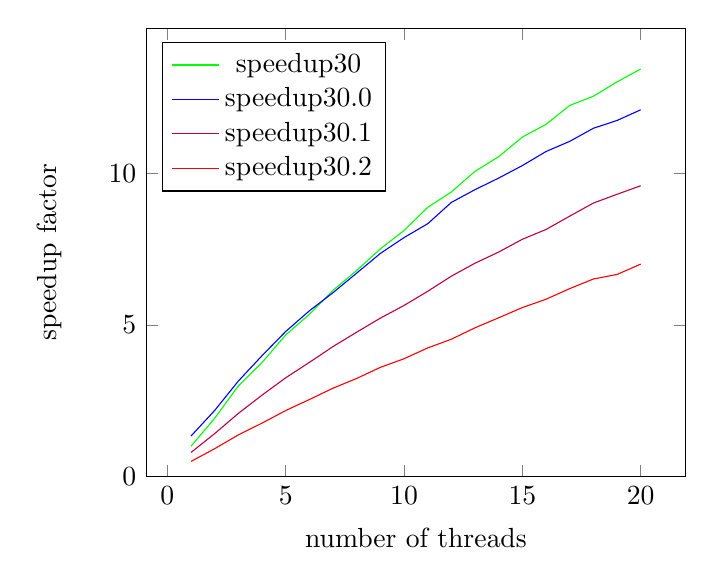
\begin{tikzpicture}
\begin{axis}[ymin=0, xlabel={number of threads}, ylabel={speedup factor}, legend pos=north west]
\addplot [color=green] coordinates {
(1,1.000) (2,1.921) (3,2.988) (4,3.757) (5,4.668) 
(6,5.347) (7,6.138) (8,6.792) (9,7.504) (10,8.108) 
(11,8.873) (12,9.380) (13,10.061) (14,10.543) (15,11.190) 
(16,11.608) (17,12.231) (18,12.535) (19,13.008) (20,13.433) 
};
\addlegendentry{speedup30}
\addplot [color=blue] coordinates {
(1,1.336) (2,2.179) (3,3.148) (4,3.984) (5,4.781) 
(6,5.462) (7,6.061) (8,6.706) (9,7.354) (10,7.876) 
(11,8.333) (12,9.036) (13,9.457) (14,9.838) (15,10.250) 
(16,10.713) (17,11.048) (18,11.479) (19,11.736) (20,12.088) 
};
\addlegendentry{speedup30.0}
\addplot [color=purple] coordinates {
(1,0.795) (2,1.416) (3,2.082) (4,2.683) (5,3.255) 
(6,3.762) (7,4.285) (8,4.759) (9,5.222) (10,5.639) 
(11,6.105) (12,6.605) (13,7.033) (14,7.400) (15,7.821) 
(16,8.144) (17,8.583) (18,9.014) (19,9.303) (20,9.585) 
};
\addlegendentry{speedup30.1}
\addplot [color=red] coordinates {
(1,0.498) (2,0.919) (3,1.373) (4,1.761) (5,2.176) 
(6,2.538) (7,2.913) (8,3.234) (9,3.599) (10,3.883) 
(11,4.239) (12,4.527) (13,4.903) (14,5.234) (15,5.570) 
(16,5.845) (17,6.194) (18,6.511) (19,6.661) (20,7.003) 
};
\addlegendentry{speedup30.2}
\end{axis}
\end{tikzpicture}
% \hspace{1cm}
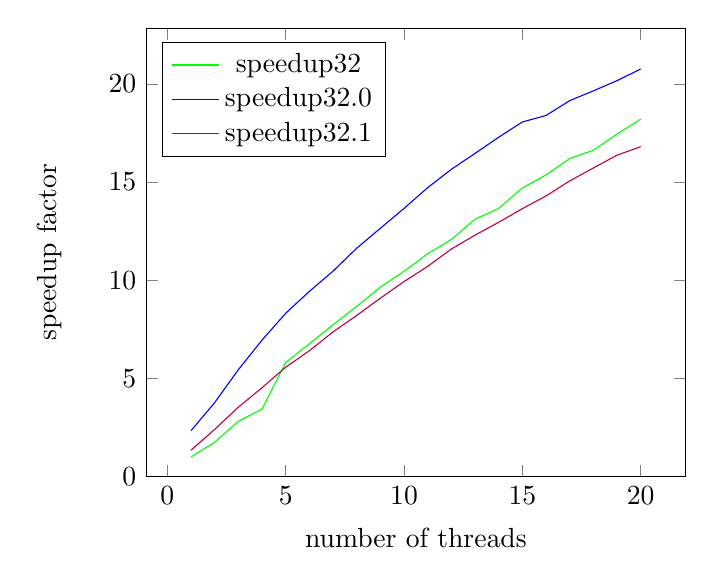
\begin{tikzpicture}
\begin{axis}[ymin=0, xlabel={number of threads}, ylabel={speedup factor}, legend pos=north west]
\addplot [color=green] coordinates {
(1,1.000) (2,1.752) (3,2.813) (4,3.439) (5,5.810) 
(6,6.762) (7,7.732) (8,8.669) (9,9.646) (10,10.460) 
(11,11.348) (12,12.077) (13,13.107) (14,13.663) (15,14.698) 
(16,15.363) (17,16.202) (18,16.623) (19,17.446) (20,18.207) 
};
\addlegendentry{speedup32}
\addplot [color=blue] coordinates {
(1,2.337) (2,3.767) (3,5.445) (4,6.949) (5,8.319) 
(6,9.432) (7,10.462) (8,11.632) (9,12.648) (10,13.658) 
(11,14.717) (12,15.652) (13,16.461) (14,17.286) (15,18.063) 
(16,18.393) (17,19.149) (18,19.647) (19,20.169) (20,20.761) 
};
\addlegendentry{speedup32.0}
\addplot [color=purple] coordinates {
(1,1.343) (2,2.404) (3,3.534) (4,4.526) (5,5.570) 
(6,6.410) (7,7.367) (8,8.208) (9,9.085) (10,9.932) 
(11,10.707) (12,11.590) (13,12.297) (14,12.954) (15,13.647) 
(16,14.294) (17,15.060) (18,15.718) (19,16.371) (20,16.804) 
};
\addlegendentry{speedup32.1}

\end{axis}
\end{tikzpicture}
\end{center}
\label{speedup}
\end{figure}

\section{Choice of graph size}
The chosen Cuckoo graph size affects what type of hardware can mine effectively at a given block interval time.
To illustrate, suppose an average desktop machine needs 1 minute for a single proof attempt,
and the block interval time is only 2 minutes. Then it will waste a large fraction (almost half)
of its attempts, as about half the time, someone else finds a proof in under 2 minutes. To reduce such waste
to a small percentage, the time for a single proof attempt should be a similarly small fraction of the block
interval time. This desirable property is known as {\em progress-freeness}, and in our case
is achieved more easily with a small graph (and hence memory) size.

Larger memory sizes have two advantages though. First, they make it harder for botnets to mine without
causing excessive swapping. Sending a computer into swap-hell will likely alert its owner and trigger a cleanup,
so botnet operators can be expected to eschew memory-intensive proofs-of-work in favor of low-memory ones.

Second, they make it harder for custom FPGA or ASIC implementations to remain self-contained.
Rather, to remain cost effective, they will likely need to make use of commodity DRAM chips,
and incur a roughly $50$ns row activation delay for random access to each memory bank.
If a future CPU with hardware siphash24 support can saturate DRAM, then there may no need
to develop ASICs (and keep them on the leading edge of process technology)
for the computational part of Cuckoo Cycle.

We expect these opposing goals to lead to graph sizes from $2^{28}$ to $2^{32}$, with the larger ones geared
more toward longer block interval times and faster mining hardware.

\section{Dynamic Sizing}
Ideally, graph size should grow with evolving memory chip capacities and cache sizes.
Although these have shown remarkable adherence to Moore's Law in the past,
this cannot be relied on for the more distant future. We therefore propose to re-evaluate the graph size
every so-many difficulty adjustments. If the difficulty target is sufficiently low, then the
graph size is deemed to have become "too easy" for existing hardware, and gets doubled.

In order to make this transition smoother and avoid severe loss of proof-of-work power,
we propose having a range of sizes allowed at any time,
namely $k$ consecutive 2-powers for some small number $k\geq 2$.
As with Myriad-coin, separate difficulty controls are maintained for each size,
adjusted so that each size accounts for roughly $\frac{1}{k}$ of all blocks.

Doubling graph sizes is then equivalent to disabling the smallest 2-power,
and enabling a new largest one, whose initial difficulty target is twice that of the previous largest.
Even if none of the hardware that was working on the smallest 2-power is repurposed for a larger size,
since this hardware only accounted for a fraction $\frac{1}{k}$ of the rewards, the loss of
proof-of-work power should be acceptable.

It remains to decide what exact form the ``difficulties too low'' condition should take.

\section{Conclusion}
Cuckoo Cycle is a novel graph-theoretic proof-of-work design that combines scalable
memory requirements with instant verifiability, and the first where
memory latency dominates the runtime\footnote{and with dynamic sizing,
will continue to do so into the distant future.}.
This narrows the mining performance gap between custom and commodity hardware and
could lead to mining costs being dominated by investments in DRAM rather than power costs.
While \cite{poelstra2014} argues that this benefits established miners who amortized
their equipment, it fails to account for a potentially larger contingent of
non-miners with already amortized equipment that can join their ranks to reduce centralization.
Resulting changes in the economics of mining are potentially beneficial but
will certainly require additional study.
More research is also needed to determine the effectiveness of GPUs and FPGAs
at running Cuckoo Cycle.

\bibliographystyle{IEEEtran}
\bibliography{cuckoo}

\lstset{language=C,basicstyle=\footnotesize}
\section{Appendix A: cuckoo.h}
\lstinputlisting{cuckoo.h}

%\section{Appendix B: cuckoo\_miner.h}
%\lstinputlisting{cuckoo_miner.h}

%\section{Appendix C: cuckoo\_miner.cpp}
%\lstinputlisting{cuckoo_miner.cpp}

\end{document}  
